%==============================================================================
\chapter{Preliminaries}
\label{chapter:preliminaries}
%==============================================================================
This chapter covers the foundation technologies used throughout the thesis.
First, Section~\ref{sec:preliminaries-semantic-technologies} gives an overview about Semantic Technologies, i.e \gls{RDF} model as a standard model for representing the data, its data partitioning mechanism and accompanying query language \gls{SPARQL}.
It also covers basic concepts of the \gls{RDF} statistical criteria definition and quality assessment introduction. 
Later, Section~\ref{sec:preliminaries-distributed-frameworks} gives an introduction to \textit{Hadoop}, its core technologies \textit{\gls{HDFS}}, \textit{MapReduce} and \textit{Apache Spark} with its libraries that have been used in the course of this thesis.

\section{Semantic Technologies}
\label{sec:preliminaries-semantic-technologies}
Originally web was considered to be a hub for sharing web pages or documents that could be understood by humans.
In addition, interlinking with other web pages or records could also be generated anywhere on the web. 
Most of this data was intended solely for human consumption.
Machines could process and show such information but did not understand it.

Semantic Web, invented by Tim Berners-Lee in 1990 is an attempt to describe and link the web content into more meaningful to the machines.




\fixme{Complete the semantic web vision and technologies}

\begin{figure*}
\centering
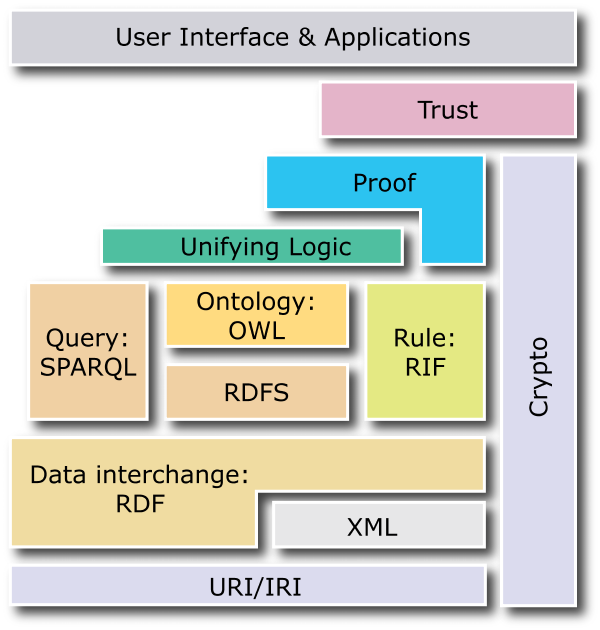
\includegraphics[width=0.7\columnwidth]{images/2_preliminaries/sw-layer-cake-2007.png}
 \caption[Semantic Web Stack]{Semantic Web Stack\footnotemark.}
\label{fig:preliminaries-sw-layer-cake}
\end{figure*}
\footnotetext{\url{https://www.w3.org/2007/03/layerCake.png} (retrieved in September 2019)}


Figure~\ref{fig:preliminaries-sw-layer-cake} depict various layers of Semantic Web related technologies, according to the \gls{W3C}.
Here we highlight \textit{Data interchange: \gls{RDF}} and \textit{Query: \gls{SPARQL}} layers, which are relevant to the work presented in this thesis and are therefore discussed in this chapter.


\subsection{RDF Data}

The Resource Description Framework (\gls{RDF}) is a \gls{W3C} standard for describing resources.
A resource is a fact or a thing which can be described and identified. 
A person, a home page, this thesis is a resource. 
An RDF resource is identified by a \gls{URI} reference.

An RDF graph is a set of RDF triples $(S,P,O)$ where $S$ is called the \emph{Subject}, $P$ is the \emph{Predicate} and $O$ is the \emph{Object}, each of which can be an \gls{URI}, subjects and objects can alternatively be blank nodes and objects can also represent literal data values.

\begin{figure*}
\centering
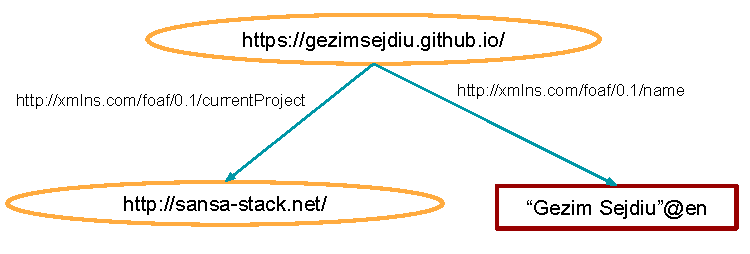
\includegraphics[width=1.0\columnwidth]{images/2_preliminaries/rdf-triple-example.pdf}
 \caption{Sample RDF Graph representation.}
\label{fig:preliminaries-rdf-graph-sample}
\end{figure*}

Figure~\ref{fig:preliminaries-rdf-graph-sample} represent an \gls{RDF} graph sample about $\verb|"Gezim Sejdiu"|$ as a resource.
An RDF triple is used to describe properties of resources and it has the following format:
$$\verb|<Subject::(resource)> <Predicate::(property)> <Object::(property value)>.|$$

Below we give some necessary notions about RDF.

\begin{definition}[RDF Term]
Let $\mathcal{U}$, be a set of URIs, $\mathcal{B}$ set of blank nodes and $\mathcal{L}$ set of literals, an RDF term ($\mathcal{T}$) is a set of $\mathcal{U} \cup \mathcal{B}\cup \mathcal{L}$.
\end{definition}

\begin{definition}[RDF Triple]
Let $\mathcal{U}$, be a set of URIs, $\mathcal{B}$ set of blank nodes and $\mathcal{L}$ set of literals, an RDF triple is a ternary tuple in the form of ${(s, p, o) \in (\mathcal{U} \cup \mathcal{B}) \times \mathcal{U} \times (U \cup B \cup L)}$, where the subject $s \in (U \cup B)$ is a resource, the predicate $p \in U$ is a property, and the object $o \in (\mathcal{U} \cup \mathcal{B} \cup \mathcal{L})$ is either another resource ($\mathcal{U} \cup \mathcal{B}$) or a literal ($\mathcal{L}$).
\end{definition}

\begin{definition}[RDF Graph]
An RDF Graph ($\mathcal{G}=\{t_1, t_2, \dots , t_n\}$) is defined as a finite set of RDF triples $t_i$.
\end{definition}

\begin{definition}[RDF Dataset]
An RDF \textit{dataset} is a collection of RDF graphs $$D = \{ G_{0},\langle i_1, G_1 \rangle, \dots , \langle i_n, G_n \rangle \}$$ where $i_1, \dots , i_n \in \mathcal{U}$.
$G_0$ is considered as a default graph which deos not have a name and can be $\emptyset$.
\end{definition}

\subsubsection{RDF Serialization Formats}

\subsection{SPARQL}

\subsection{RDF Statistics}
In this section we define a statistical criteria
\begin{definition}[Statistical criteria]\cite{demter-2012-ekaw}
\label{def:preliminaries-statistics}
A statistical criterion is a triple $(F,D,P)$, where: \vspace{-5pt}
\begin{itemize}
	\item $F$ is a SPARQL filter condition.
	\item $D$ is a data structure for storing intermediate results and a description how to fill this data structure with values from the triple stream after applying $F$.
	\item $P$ is a post-processing filter operating on the data structure $D$.
\end{itemize} \vspace{-5pt}
\end{definition}

\subsection{RDF quality assessment}

\section{Hadoop Ecosystem}
\label{sec:preliminaries-distributed-frameworks}
Apache Hadoop~\cite{White:2015:HDG:2904397} is a collection of distributed processing and storage frameworks of large-scale datasets across a cluster of computers.
Its ecosystem contains a build-in mechanisms in order to guarantee fault tolerance and high availability in addition to commodity hardware.
Therefore, specific hardware involvement is not needed, making it highly scalable and cost-effective.

As of today, Hadoop ecosystem has been enriched with an extensive tools and libraries that are either built on top of Hadoop or use it for different application fields, including but not limited to: data mining, querying, data analysis, processing and data warehousing.
It has become the de-facto industry standard in the Big Data management all thanks to its high degree of parallelism, fault-tolerant, reliability and scalability.

In this section, we provide a brief overview of the Hadoop ecosystem projects used in the course of this thesis.
We concentrate mostly on the elements needed to comprehend the content of the following chapters without going into the technical details.

\subsection{Apache Hadoop and MapReduce}

\subsubsection{HDFS}
The Hadoop Distributed File System (\gls{HDFS})~\cite{Shvachko:2010:HDF:1913798.1914427} is one of the main components of the Hadoop. 
It is a popular file system capable of of handling the distribution of the data across multiple nodes in the cluster.
HDFS serve as a common, distributed and fault-tolerant data lake for all applications on top of the Hadoop in order to minimize the data movement and duplication.
Furthermore, it also leverage the distributed processing of large-scale datasets by adapting advanced and automatically partitioning techniques across all the nodes in the cluster.
\gls{HDFS} was originally built as infrastructure for the Apache Nutch\furl{https://nutch.apache.org/} web search engine project and was inspired by the \gls{GFS}~\cite{Ghemawat:2003:GFS:945445.945450}. 
\gls{HDFS} is part of the Apache Hadoop ecosystem.

\gls{HDFS} is designed in a way that it doesn't require highly reliable and costly hardware but instead, it can be run on a cluster of computers with commodity hardware.



\subsubsection{MapReduce}
Beside its distributed file system, Hadoop contains computing system so-called MapReduce.
MapReduce is a distributed framework that allows for the distributed processing of large data sets across a cluster of computers.  

%\framebox[1.1\width]{\texttt{Step 3}}

\subsection{Apache Spark}
Apache Spark is a fast and generic-purpose cluster computing engine which is built over the Hadoop ecosystem.
\gls{RDD}~\cite{zaharia2012resilient} which are a fault-tolerant and immutable collections of records that can be operated in a parallel setting.
Apache Spark provides a rich set of APIs for faster, in-memory processing of RDDs. 